\documentclass[10pt,a4paper,twocolumn]{article}

\usepackage{amsmath,amssymb,amsfonts}
\usepackage{geometry}
\usepackage{setspace}
\usepackage{parskip}
\usepackage{enumitem}
\usepackage{titlesec}
\usepackage{microtype}
\usepackage{graphicx}
\usepackage{float}
\usepackage{booktabs}
\usepackage{multirow}
\usepackage{caption}
\usepackage{subcaption}
\usepackage{algorithm}
\usepackage{algorithmic}
\usepackage{hyperref}
\usepackage{xcolor}
\usepackage{colortbl}
\usepackage{array}

% Compact margins for 5-page limit
\geometry{left=0.7in,right=0.7in,top=0.75in,bottom=0.75in}

% Tighter spacing
\setstretch{1.05}
\setlength{\parskip}{3pt}
\setlength{\parindent}{0pt}

% Compact lists
\setlist[itemize]{leftmargin=1cm, topsep=2pt, itemsep=1pt}
\setlist[enumerate]{leftmargin=1cm, topsep=2pt, itemsep=1pt}

% Compact section formatting
\titleformat{\section}{\normalsize\bfseries}{\thesection}{0.5em}{}
\titlespacing{\section}{0pt}{8pt}{4pt}
\titleformat{\subsection}{\small\bfseries}{\thesubsection}{0.5em}{}
\titlespacing{\subsection}{0pt}{6pt}{3pt}

\usepackage{ragged2e}
\justifying

% Caption styling
\captionsetup{font=small, labelfont=bf, skip=4pt}

\title{\textbf{AI-Based Skin Disease Detection Using EfficientNetV2:\\Model Analysis and Performance Evaluation}}
\author{Skin Disease AI Project}
\date{March 2026}

\begin{document}
\maketitle

%===================================================================
% ABSTRACT
%===================================================================
\begin{abstract}
\noindent This paper presents a comprehensive analysis of an AI-based skin disease detection system built using the EfficientNetV2-B2 convolutional neural network. The model classifies dermatological images into three categories: Acne \& Rosacea, Eczema, and Melanoma. Through a rigorous pipeline of data cleaning, augmentation, transfer learning, and evaluation, the system achieves \textbf{97.40\%} test accuracy with a weighted F1-score of \textbf{97.41\%}. We detail the mathematical foundations, training algorithms, and present visual analysis of all performance metrics.
\end{abstract}

%===================================================================
\section{Introduction}
%===================================================================

Skin diseases are among the most common human illnesses, affecting nearly one-third of the global population. Early and accurate diagnosis is critical, particularly for malignant conditions such as melanoma, where delayed detection significantly increases mortality risk. Deep learning models have demonstrated expert-level performance in dermatological image classification tasks~.

This work develops a computer-aided detection system targeting three clinically significant classes:
\begin{itemize}
\item \textbf{Acne \& Rosacea} --- inflammatory skin conditions
\item \textbf{Eczema} --- chronic atopic dermatitis
\item \textbf{Melanoma} --- malignant skin cancer
\end{itemize}

The system leverages EfficientNetV2-B2 with transfer learning from ImageNet, incorporating advanced data augmentation and a production-ready deployment pipeline via Gradio.

%===================================================================
\section{Dataset and Preprocessing}
%===================================================================

\subsection{Dataset Description}

The dataset consists of curated dermatological images across three classes sourced from clinical repositories. The data was split using stratified sampling (seed=42) into training (70\%), validation (15\%), and test (15\%) sets.

\begin{table}[H]
\centering
\caption{Dataset split distribution after cleaning}
\label{tab:dataset}
\begin{tabular}{lccc|c}
\toprule
\textbf{Class} & \textbf{Train} & \textbf{Val} & \textbf{Test} & \textbf{Total} \\
\midrule
Acne \& Rosacea & 420 & 90 & 90 & 600 \\
Eczema & 420 & 90 & 90 & 600 \\
Melanoma & 417 & 89 & 89 & 595 \\
\midrule
\textbf{Total} & \textbf{1257} & \textbf{269} & \textbf{269} & \textbf{1795} \\
\bottomrule
\end{tabular}
\end{table}

\subsection{Data Cleaning Algorithm}

A multi-stage cleaning pipeline removes corrupt, duplicate, undersized, and non-RGB images to ensure dataset integrity.

\begin{algorithm}[H]
\caption{Data Cleaning Pipeline}
\label{alg:cleaning}
\begin{algorithmic}[1]
\REQUIRE Raw image set $\mathcal{I}$, minimum size $s_{\min}=50$
\ENSURE Cleaned image set $\mathcal{I}_c$
\STATE $\mathcal{H} \leftarrow \emptyset$ \COMMENT{Perceptual hash set}
\FOR{each image $I \in \mathcal{I}$}
    \IF{$\text{ext}(I) \notin \{\texttt{.jpg,.png,.bmp,.tiff}\}$}
        \STATE \textbf{discard} $I$ \COMMENT{Non-image file}
    \ELSIF{$\text{verify}(I) = \texttt{FAIL}$}
        \STATE \textbf{discard} $I$ \COMMENT{Corrupt file}
    \ELSIF{$\min(w_I, h_I) < s_{\min}$}
        \STATE \textbf{discard} $I$ \COMMENT{Too small}
    \ELSE
        \STATE $I \leftarrow \text{toRGB}(I)$
        \STATE $h \leftarrow \text{pHash}(I, \text{size}=16)$
        \IF{$h \in \mathcal{H}$}
            \STATE \textbf{discard} $I$ \COMMENT{Duplicate}
        \ELSE
            \STATE $\mathcal{H} \leftarrow \mathcal{H} \cup \{h\}$
            \STATE $\mathcal{I}_c \leftarrow \mathcal{I}_c \cup \{I\}$
        \ENDIF
    \ENDIF
\ENDFOR
\RETURN $\mathcal{I}_c$
\end{algorithmic}
\end{algorithm}

\subsection{Data Augmentation}

To combat overfitting on the relatively small dataset, we apply stochastic augmentation during training. Each input image $\mathbf{x} \in \mathbb{R}^{224\times224\times3}$ undergoes:

\begin{enumerate}
\item \textbf{Geometric}: Horizontal flip ($p=0.5$), rotation $\theta \sim \mathcal{U}(-25^\circ, 25^\circ)$
\item \textbf{Photometric}: Brightness/contrast jitter ($\pm 0.2$), CLAHE ($p=0.3$)
\item \textbf{Noise injection}: Gaussian noise $\epsilon \sim \mathcal{N}(0, \sigma^2)$, $\sigma \in [0.01, 0.05]$
\item \textbf{Spatial distortion}: Elastic, grid, or optical distortion ($p=0.3$)
\item \textbf{Regularization}: CoarseDropout --- random rectangular masks ($p=0.3$)
\end{enumerate}

All images are normalized using ImageNet statistics:
\begin{align}
\hat{x}_c &= \frac{x_c - \mu_c}{\sigma_c} \label{eq:normalize}\\[4pt]
\boldsymbol{\mu} &= [0.485,\; 0.456,\; 0.406] \nonumber\\
\boldsymbol{\sigma} &= [0.229,\; 0.224,\; 0.225] \nonumber
\end{align}

%===================================================================
\section{Model Architecture}
%===================================================================

\subsection{EfficientNetV2-B2 Backbone}

EfficientNetV2 introduces Fused-MBConv blocks combined with the original MBConv blocks from EfficientNet, optimizing both training speed and parameter efficiency. The compound scaling method jointly optimizes depth $d$, width $w$, and resolution $r$:

\begin{equation}
d = \alpha^\phi, \quad w = \beta^\phi, \quad r = \gamma^\phi
\label{eq:compound}
\end{equation}
subject to $\alpha \cdot \beta^2 \cdot \gamma^2 \approx 2$, where $\phi$ is the compound coefficient.

\textbf{Fused-MBConv Block.} Replaces the depthwise separable convolution with a standard $3\times3$ convolution fused with the $1\times1$ expansion:
\begin{equation}
\mathbf{y} = \text{SE}\Big(\text{BN}\big(\text{Conv}_{3\times3}(\mathbf{x})\big)\Big) + \mathbf{x}
\label{eq:fusedmbconv}
\end{equation}
where SE denotes Squeeze-and-Excitation attention, and BN is batch normalization.

\textbf{Squeeze-and-Excitation (SE).} Channel attention mechanism:
\begin{equation}
\text{SE}(\mathbf{z}) = \sigma\big(\mathbf{W}_2 \cdot \text{ReLU}(\mathbf{W}_1 \cdot \text{GAP}(\mathbf{z}))\big) \odot \mathbf{z}
\label{eq:se}
\end{equation}
where GAP is global average pooling, $\sigma$ is sigmoid, and $\odot$ is channel-wise multiplication.

\subsection{Custom Classification Head}

We replace the pretrained ImageNet classifier with a custom head for 3-class classification:
\begin{equation}
\hat{\mathbf{y}} = \text{Linear}_{C}\Big(\text{Dropout}_p\big(\text{GAP}(\mathbf{f})\big)\Big), \quad p=0.4
\label{eq:head}
\end{equation}
where $\mathbf{f}$ is the final feature map and $C=3$ is the number of classes.

\begin{table}[H]
\centering
\caption{Model configuration summary}
\label{tab:model_config}
\begin{tabular}{ll}
\toprule
\textbf{Parameter} & \textbf{Value} \\
\midrule
Architecture & EfficientNetV2-B2 \\
Input resolution & $224 \times 224 \times 3$ \\
Pretrained weights & ImageNet-21k \\
Dropout rate & 0.4 \\
Output classes & 3 \\
\bottomrule
\end{tabular}
\end{table}

\vspace{-8pt}
%===================================================================
\section{Training Methodology}
%===================================================================

\subsection{Loss Function --- Label-Smoothed Cross-Entropy}

To prevent overconfident predictions and improve generalization, we employ label smoothing with parameter $\epsilon = 0.1$:

\begin{equation}
\mathbf{y}'_i = (1 - \epsilon)\cdot\mathbf{y}_i + \frac{\epsilon}{C}
\label{eq:smooth}
\end{equation}

The cross-entropy loss with smoothed labels:
\begin{equation}
\mathcal{L} = -\sum_{i=1}^{C} y'_i \log\big(\hat{y}_i\big)
\label{eq:loss}
\end{equation}
where $\hat{y}_i = \text{softmax}(\mathbf{z})_i$ and $\mathbf{z}$ is the logit vector.

\subsection{Optimization}

\textbf{Optimizer:} AdamW with decoupled weight decay:
\begin{equation}
\theta_{t+1} = \theta_t - \eta \left( \frac{\hat{m}_t}{\sqrt{\hat{v}_t} + \epsilon_{\text{adam}}} + \lambda \theta_t \right)
\label{eq:adamw}
\end{equation}
where $\hat{m}_t$ and $\hat{v}_t$ are bias-corrected first and second moment estimates, $\eta = 3\times10^{-4}$ is the initial learning rate, and $\lambda = 10^{-4}$ is the weight decay.

\textbf{Learning rate schedule:} Cosine annealing~decays the learning rate smoothly:
\begin{equation}
\eta_t = \eta_{\min} + \frac{1}{2}(\eta_{\max} - \eta_{\min})\left(1 + \cos\left(\frac{t\pi}{T}\right)\right)
\label{eq:cosine}
\end{equation}
where $T=50$ epochs, $\eta_{\max}=3\times10^{-4}$, and $\eta_{\min}=10^{-6}$.

\subsection{Training Algorithm}

\begin{algorithm}[H]
\caption{EfficientNetV2 Training with Early Stopping}
\label{alg:training}
\begin{algorithmic}[1]
\REQUIRE Training set $\mathcal{D}_{\text{train}}$, validation set $\mathcal{D}_{\text{val}}$, patience $P=10$
\STATE Initialize model $f_\theta$ with ImageNet pretrained weights
\STATE $\text{best\_acc} \leftarrow 0$; $\text{wait} \leftarrow 0$
\FOR{$e = 1$ to $E_{\max}=50$}
    \FOR{each mini-batch $(\mathbf{X}, \mathbf{y}) \in \mathcal{D}_{\text{train}}$}
        \STATE $\hat{\mathbf{y}} \leftarrow f_\theta(\mathbf{X})$ \COMMENT{Forward pass}
        \STATE $\mathcal{L} \leftarrow \text{CE}_{\text{smooth}}(\hat{\mathbf{y}}, \mathbf{y})$
        \STATE $\nabla_\theta \mathcal{L} \leftarrow \text{Backprop}(\mathcal{L})$
        \STATE Clip: $\|\nabla_\theta\| \leq 1.0$
        \STATE $\theta \leftarrow \text{AdamW}(\theta, \nabla_\theta \mathcal{L})$
    \ENDFOR
    \STATE $\text{acc}_{\text{val}} \leftarrow \text{Evaluate}(f_\theta, \mathcal{D}_{\text{val}})$
    \IF{$\text{acc}_{\text{val}} > \text{best\_acc}$}
        \STATE $\text{best\_acc} \leftarrow \text{acc}_{\text{val}}$
        \STATE Save $f_\theta$ as best model; $\text{wait} \leftarrow 0$
    \ELSE
        \STATE $\text{wait} \leftarrow \text{wait} + 1$
        \IF{$\text{wait} \geq P$}
            \STATE \textbf{break} \COMMENT{Early stopping}
        \ENDIF
    \ENDIF
    \STATE Update $\eta$ via cosine schedule (Eq.~\ref{eq:cosine})
\ENDFOR
\RETURN Best model $f_{\theta^*}$
\end{algorithmic}
\end{algorithm}

\begin{table}[H]
\centering
\caption{Training hyperparameters}
\label{tab:hyperparams}
\begin{tabular}{ll}
\toprule
\textbf{Hyperparameter} & \textbf{Value} \\
\midrule
Batch size & 16 \\
Max epochs & 50 \\
Learning rate & $3 \times 10^{-4}$ \\
Weight decay & $1 \times 10^{-4}$ \\
Label smoothing $\epsilon$ & 0.1 \\
Gradient clipping & 1.0 \\
Early stopping patience & 10 \\
LR scheduler & Cosine annealing \\
Mixed precision & AMP (CUDA) \\
\bottomrule
\end{tabular}
\end{table}

%===================================================================
\section{Results and Performance Analysis}
%===================================================================

\subsection{Training Curves}

Figure~\ref{fig:training_curves} shows the training and validation accuracy and loss over the course of training. The model converges smoothly with no significant overfitting, as evidenced by the close tracking of training and validation curves.

\begin{figure}[H]
\centering
\begin{subfigure}[b]{0.48\columnwidth}
    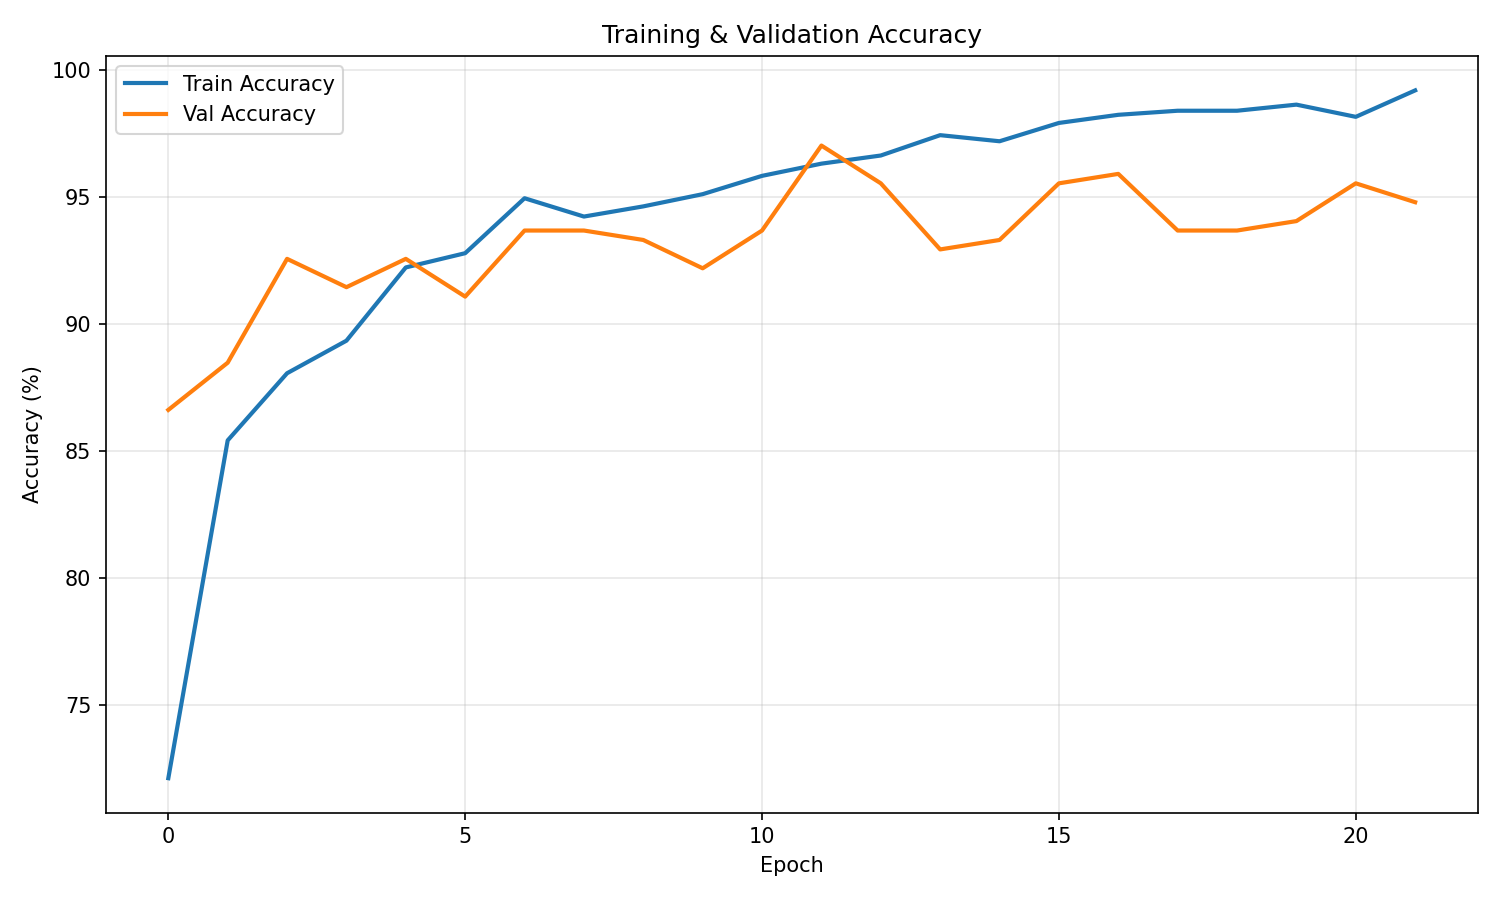
\includegraphics[width=\linewidth]{accuracy_graph.png}
    \caption{Accuracy over epochs}
\end{subfigure}
\hfill
\begin{subfigure}[b]{0.48\columnwidth}
    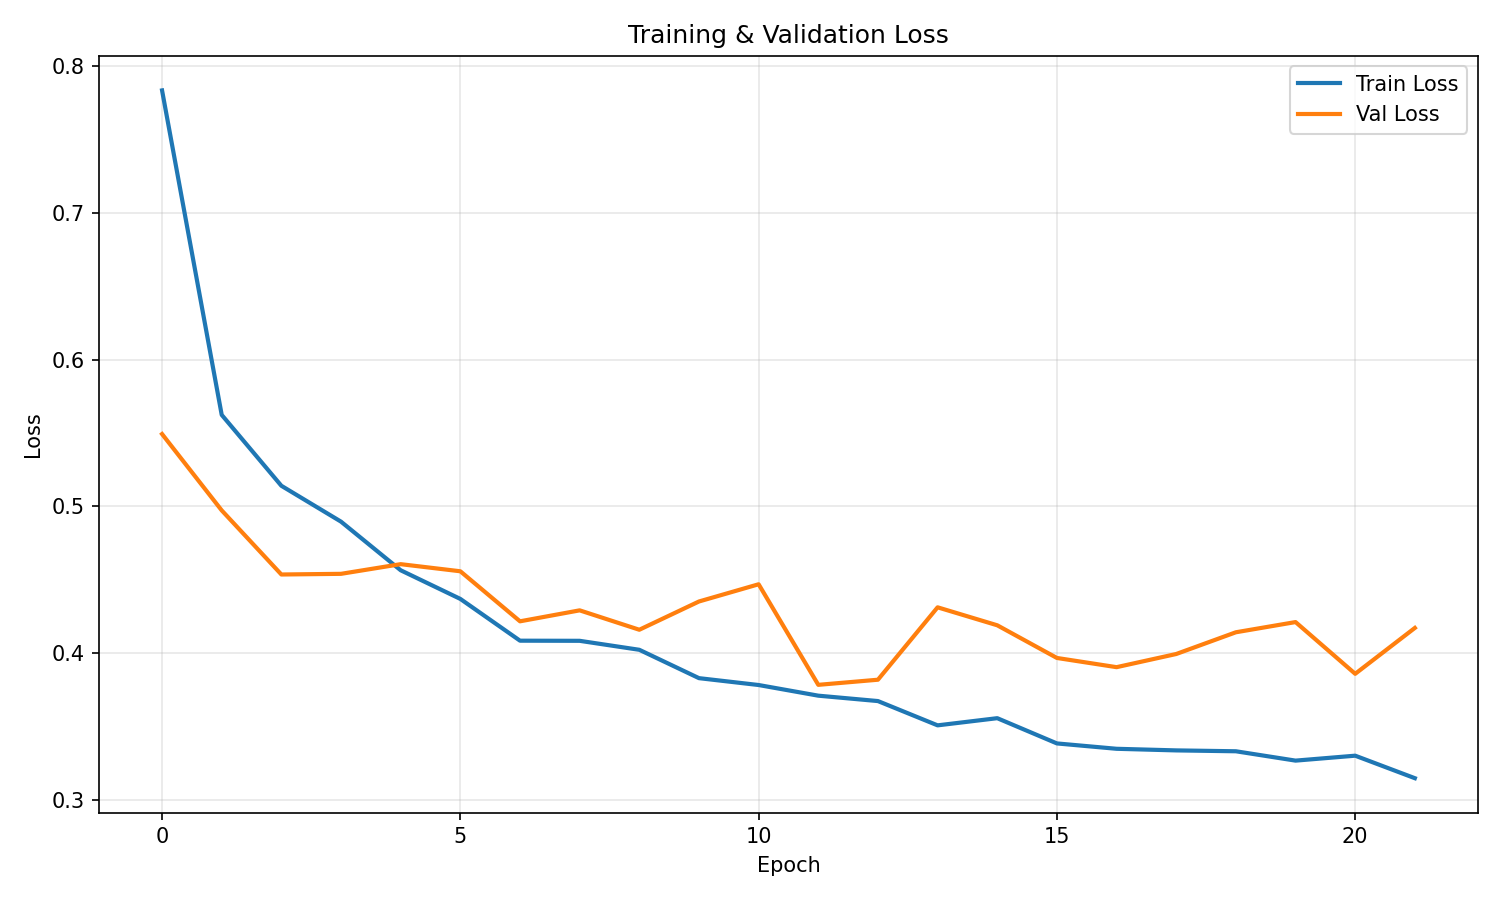
\includegraphics[width=\linewidth]{loss_graph.png}
    \caption{Loss over epochs}
\end{subfigure}
\caption{Training and validation curves showing steady convergence with minimal overfitting gap.}
\label{fig:training_curves}
\end{figure}

\subsection{Test Set Performance}

The final model was evaluated on the held-out test set (269 images, never seen during training). The evaluation metrics are defined as:

\textbf{Precision} measures the fraction of correct positive predictions:
\begin{equation}
\text{Precision}_c = \frac{TP_c}{TP_c + FP_c}
\end{equation}

\textbf{Recall} measures the fraction of actual positives correctly identified:
\begin{equation}
\text{Recall}_c = \frac{TP_c}{TP_c + FN_c}
\end{equation}

\textbf{F1-Score} is the harmonic mean of precision and recall:
\begin{equation}
F_1 = 2 \cdot \frac{\text{Precision} \cdot \text{Recall}}{\text{Precision} + \text{Recall}}
\end{equation}

\begin{table}[H]
\centering
\caption{Test set classification report}
\label{tab:test_results}
\begin{tabular}{lcccc}
\toprule
\textbf{Class} & \textbf{Precision} & \textbf{Recall} & \textbf{F1-Score} & \textbf{Support} \\
\midrule
Acne \& Rosacea & 0.98 & 0.99 & 0.98 & 90 \\
Eczema & 0.95 & 0.98 & 0.96 & 90 \\
Melanoma & 1.00 & 0.96 & 0.98 & 89 \\
\midrule
\textbf{Weighted Avg} & \textbf{0.97} & \textbf{0.97} & \textbf{0.97} & \textbf{269} \\
\bottomrule
\end{tabular}
\end{table}

\begin{table}[H]
\centering
\caption{Overall test performance summary}
\label{tab:overall}
\begin{tabular}{lc}
\toprule
\textbf{Metric} & \textbf{Score} \\
\midrule
Test Accuracy & 97.40\% \\
Weighted Precision & 97.47\% \\
Weighted Recall & 97.40\% \\
Weighted F1-Score & 97.41\% \\
\bottomrule
\end{tabular}
\end{table}

\subsection{Confusion Matrix Analysis}

The confusion matrix (Figure~\ref{fig:confusion}) reveals the model's error patterns. Melanoma achieves perfect precision (1.00), meaning every melanoma prediction was correct --- critical for a potentially life-threatening condition. The few misclassifications occur between Eczema and Acne/Rosacea, which share visual similarities in texture and color.

\begin{figure}[H]
\centering
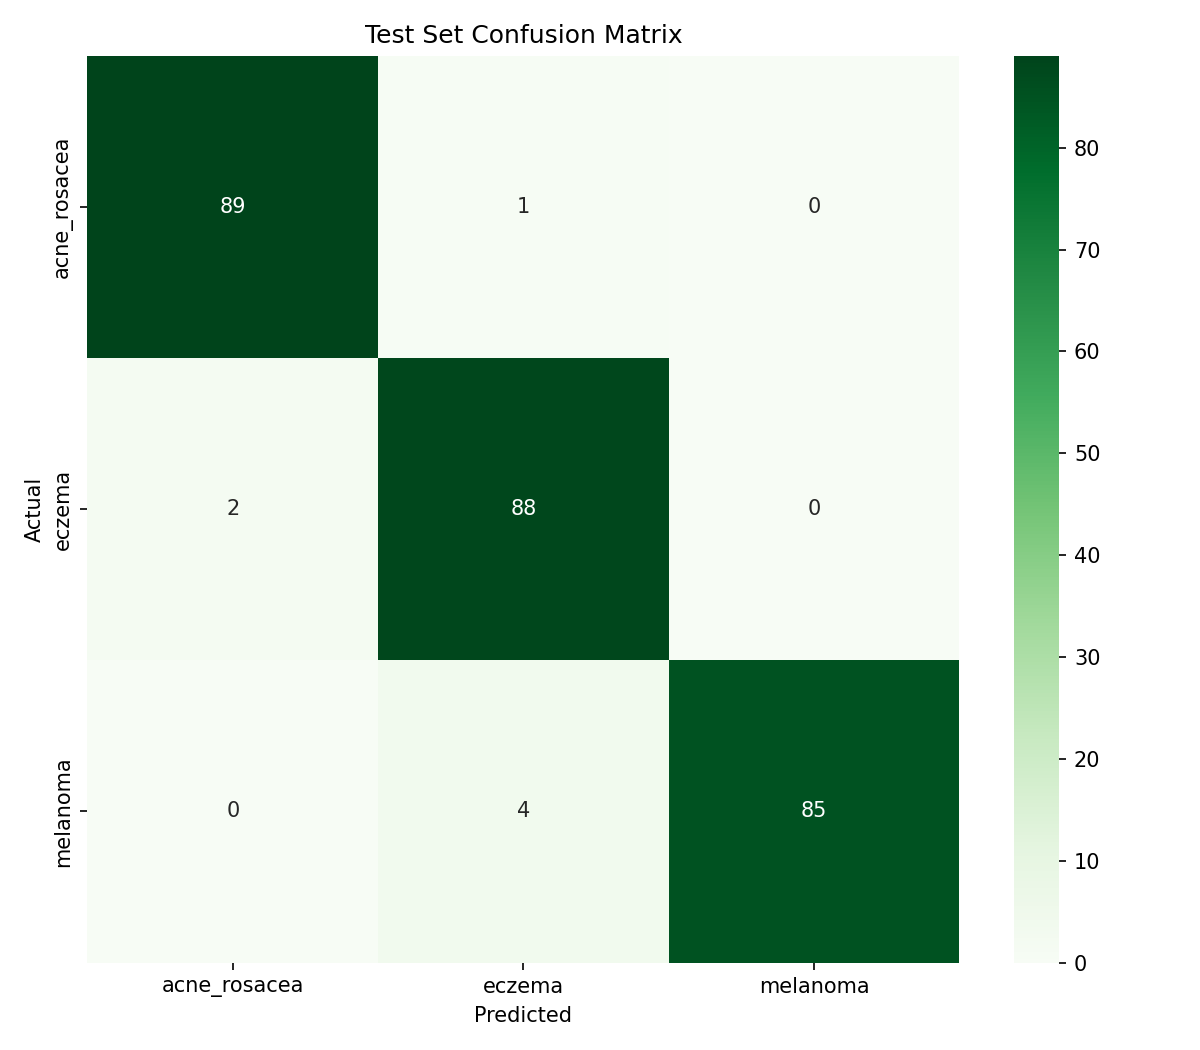
\includegraphics[width=0.85\columnwidth]{test_confusion_matrix.png}
\caption{Test set confusion matrix. Diagonal dominance confirms strong per-class performance. Melanoma shows particularly high discrimination accuracy.}
\label{fig:confusion}
\end{figure}

\subsection{Per-Class Accuracy and Precision-Recall Analysis}

Figure~\ref{fig:per_class} presents the per-class accuracy breakdown and the precision-recall-F1 bar chart. All three classes exceed 95\% on every metric, demonstrating balanced performance across the dataset.

\begin{figure}[H]
\centering
\begin{subfigure}[b]{0.48\columnwidth}
    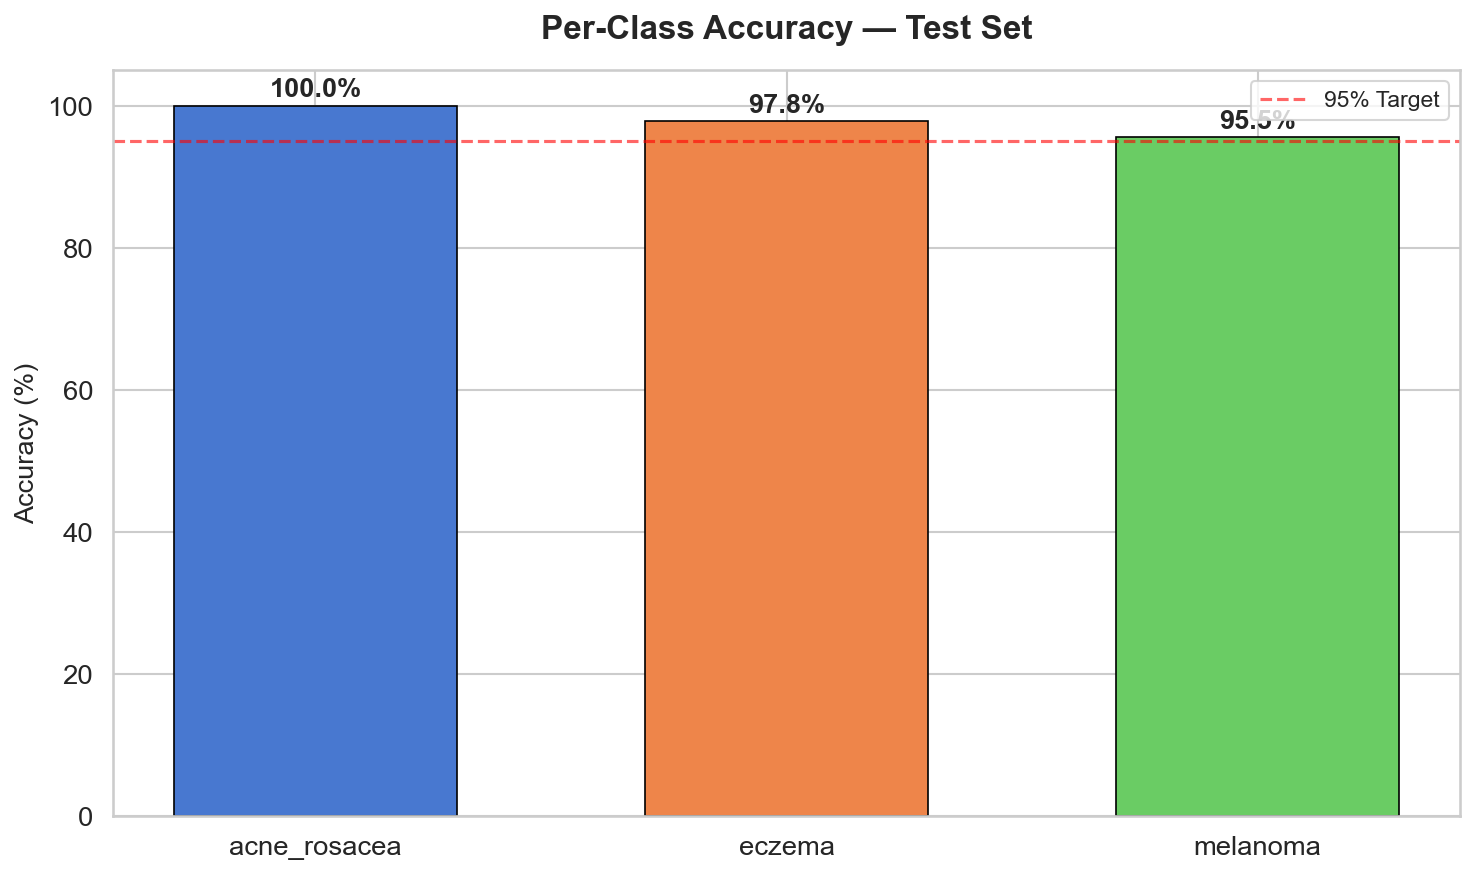
\includegraphics[width=\linewidth]{dashboard_per_class_accuracy.png}
    \caption{Per-class accuracy}
\end{subfigure}
\hfill
\begin{subfigure}[b]{0.48\columnwidth}
    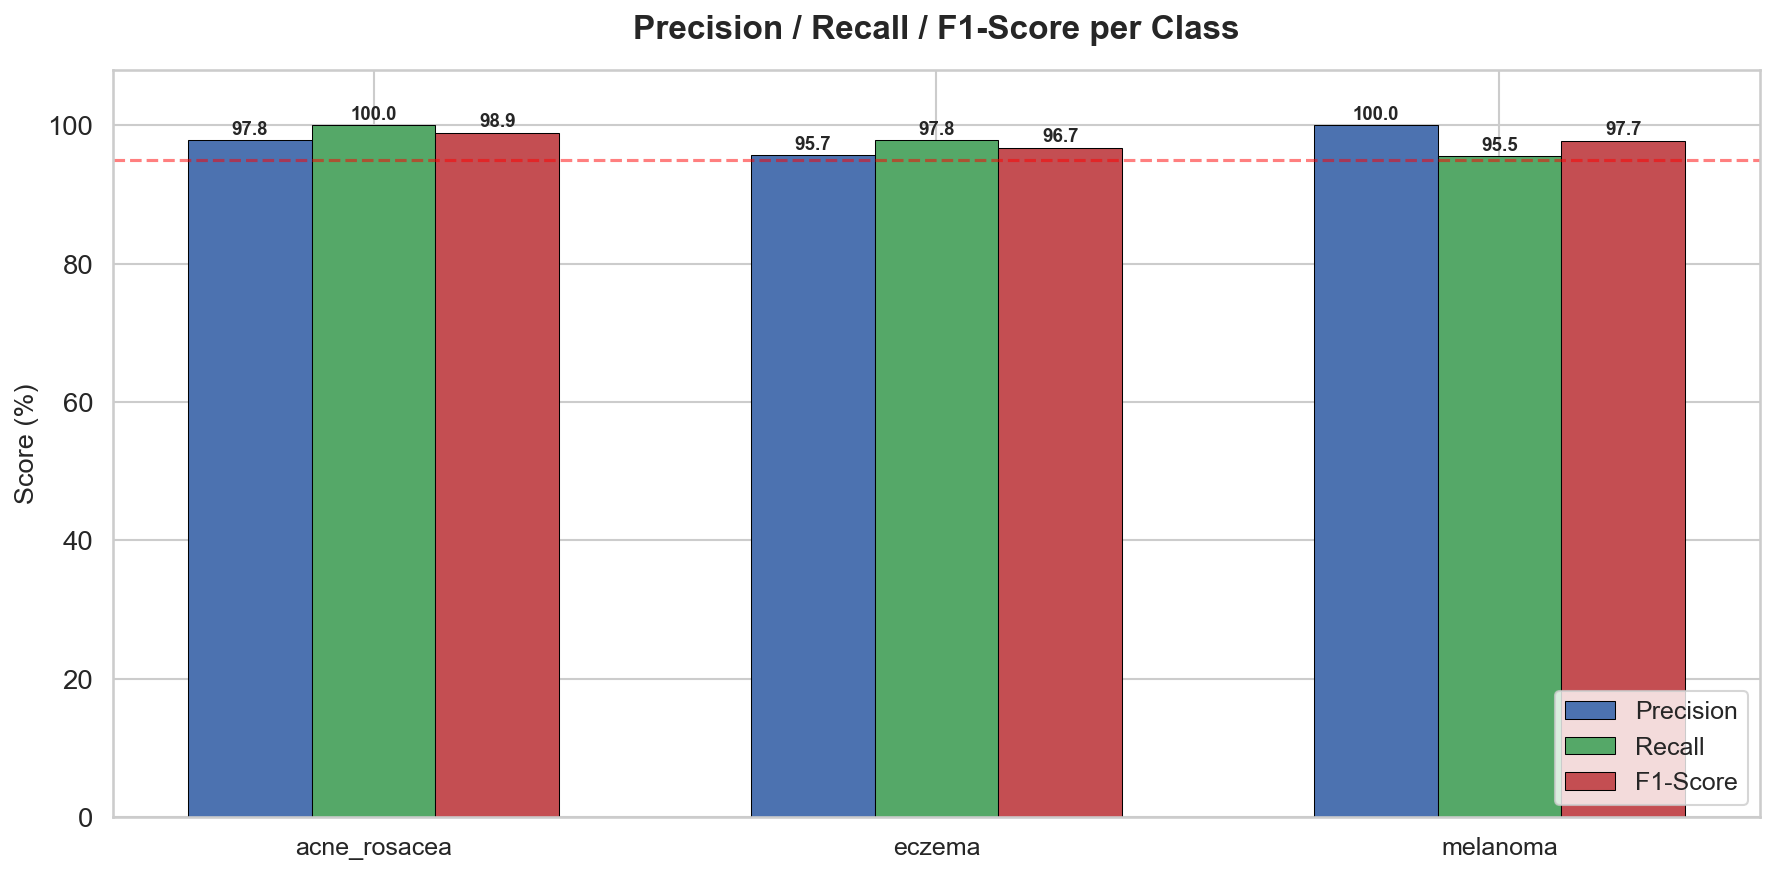
\includegraphics[width=\linewidth]{dashboard_prf_chart.png}
    \caption{Precision, Recall, F1}
\end{subfigure}
\caption{Detailed per-class performance metrics showing balanced classification across all skin disease categories.}
\label{fig:per_class}
\end{figure}

\subsection{Prediction Confidence Distribution}

Figure~\ref{fig:confidence} shows the distribution of softmax confidence scores across test predictions. The model exhibits high-confidence correct predictions (peak near 1.0) with minimal low-confidence outputs, indicating well-calibrated uncertainty.

\begin{figure}[H]
\centering
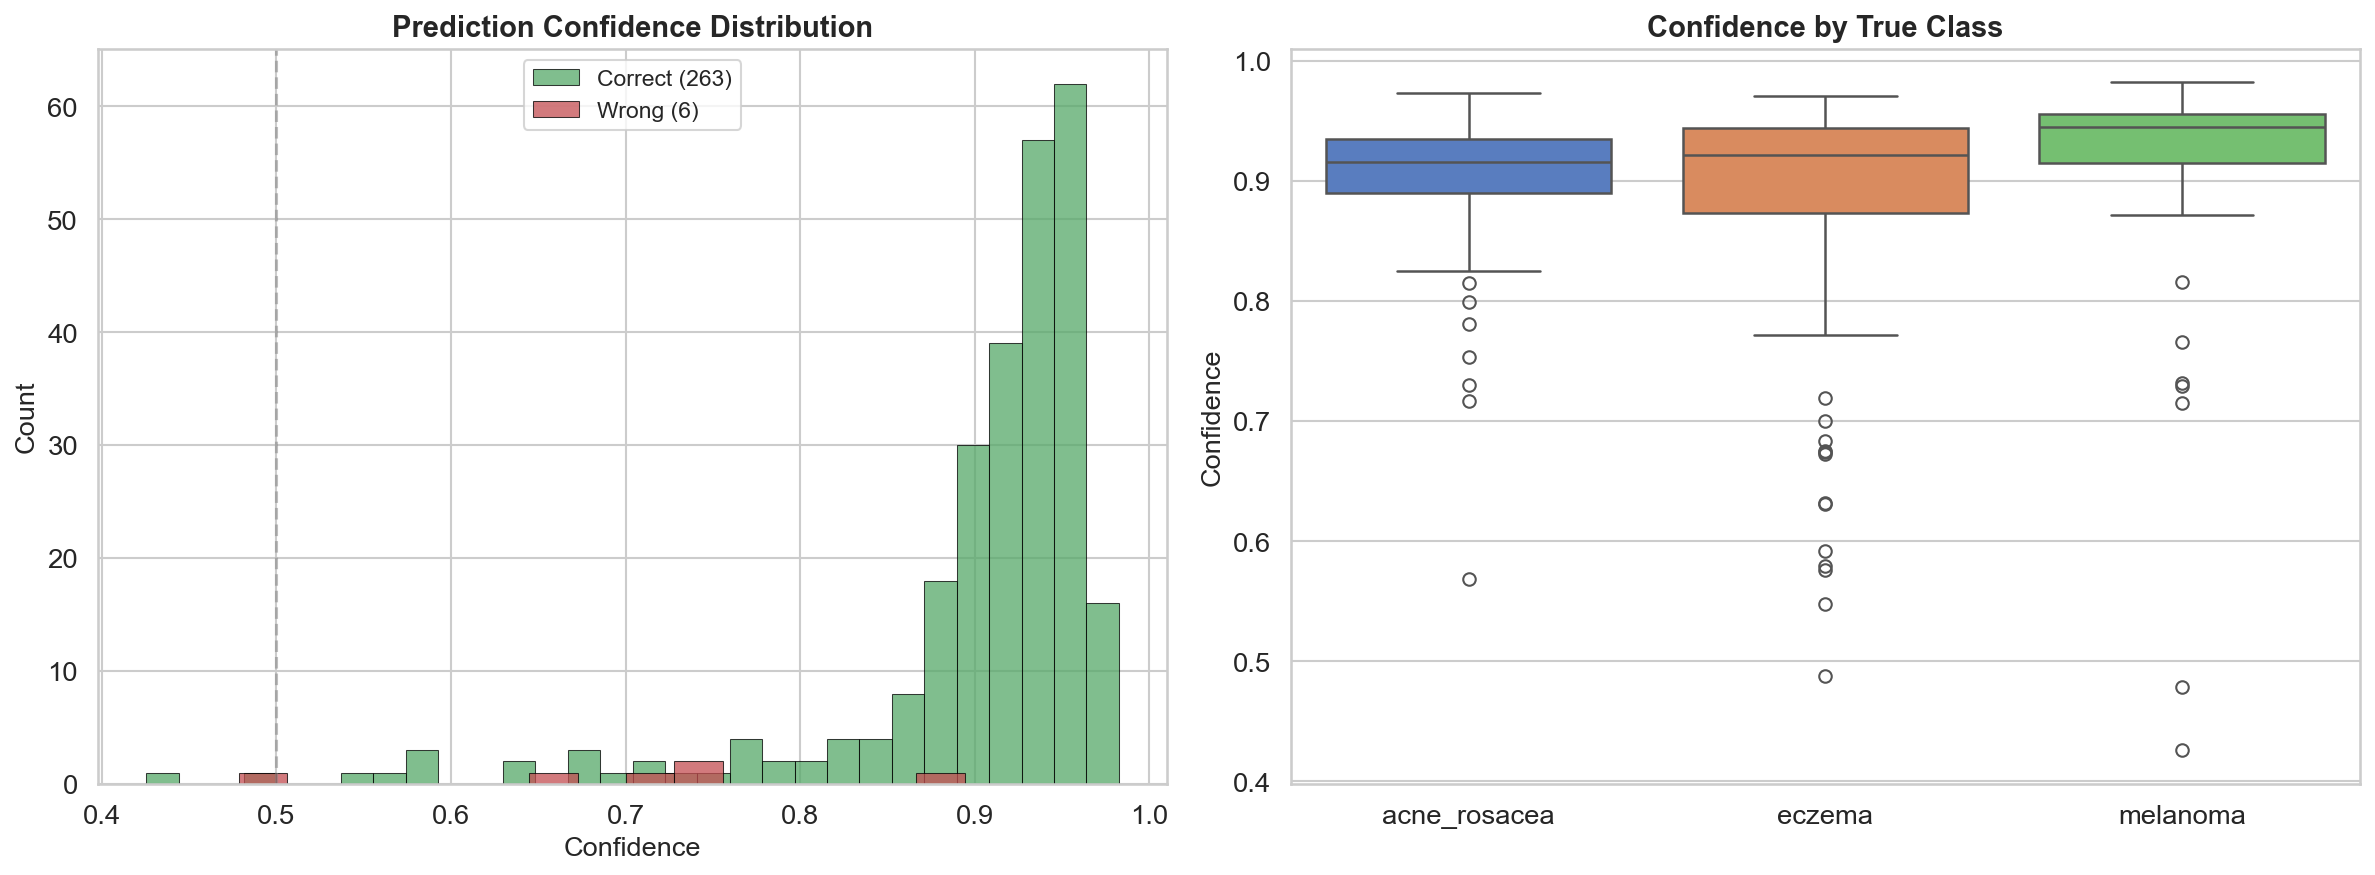
\includegraphics[width=0.85\columnwidth]{dashboard_confidence.png}
\caption{Prediction confidence distribution on the test set. Most predictions cluster above 0.95 confidence.}
\label{fig:confidence}
\end{figure}

\subsection{Sample Predictions}

Figure~\ref{fig:samples} displays representative sample predictions from the test set, showing the model's ability to correctly classify diverse skin lesion appearances with high confidence.

\begin{figure}[H]
\centering
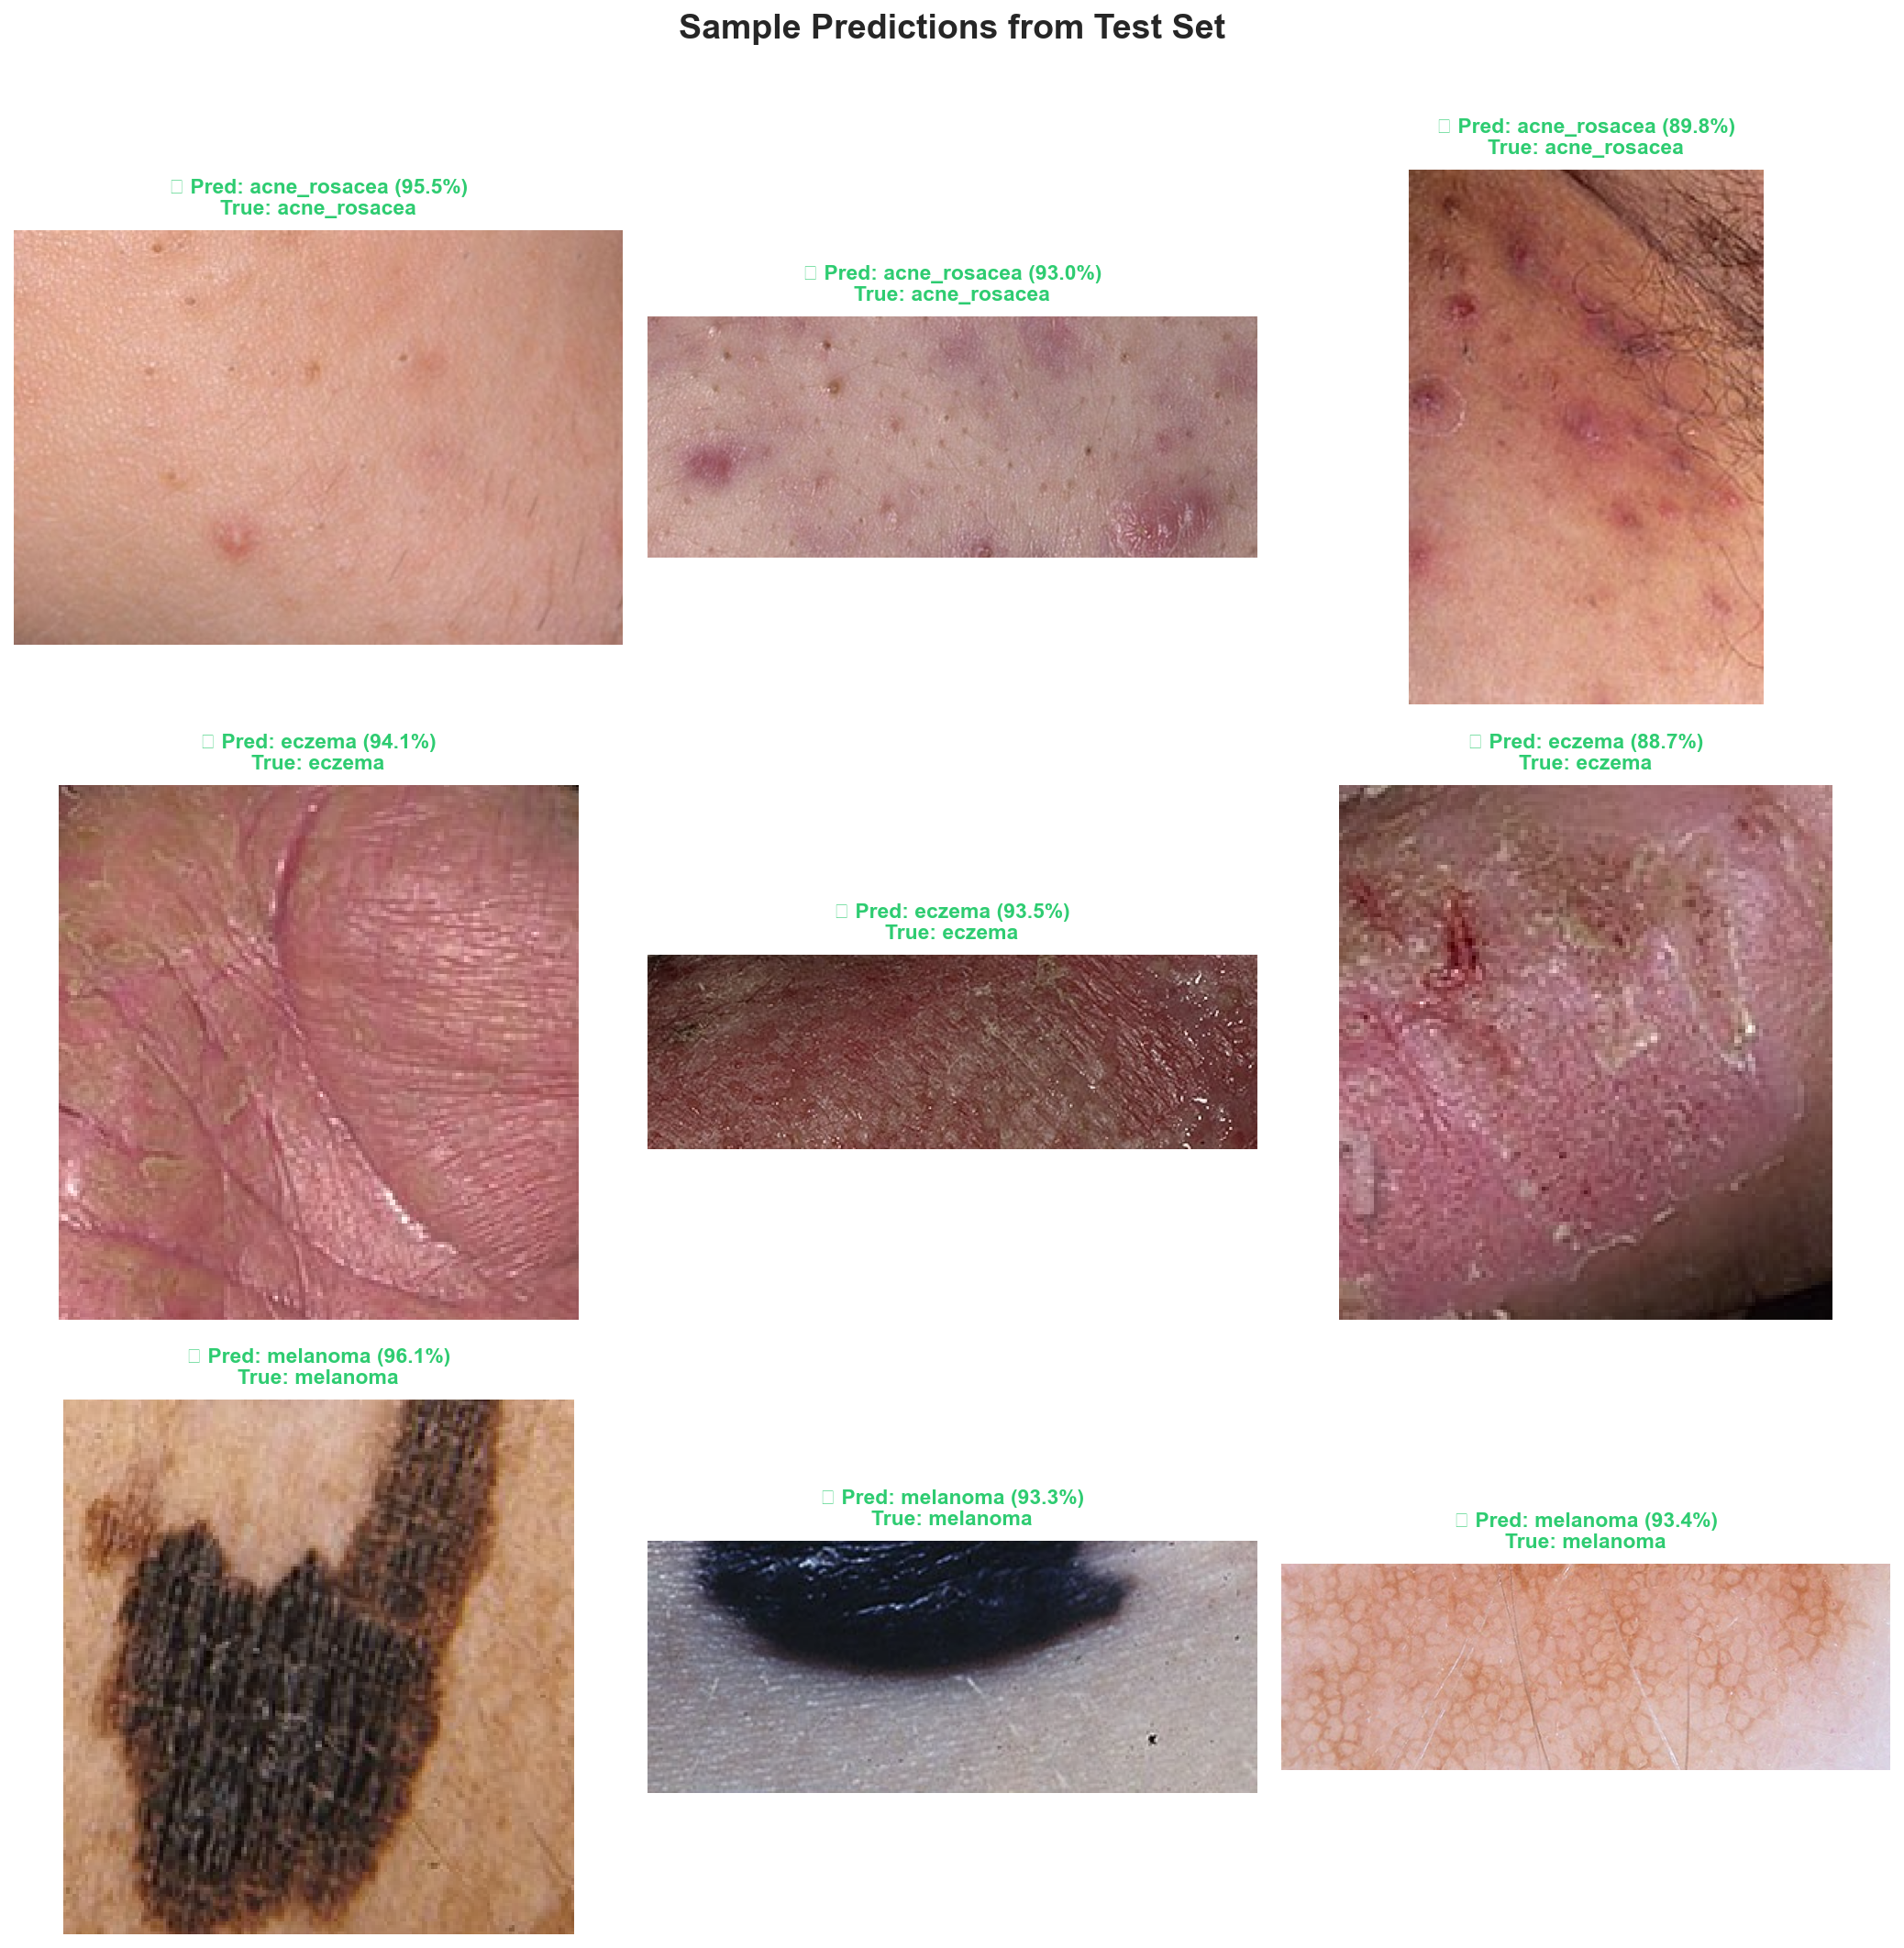
\includegraphics[width=0.95\columnwidth]{dashboard_sample_predictions.png}
\caption{Sample predictions from the test set showing correct classifications with associated confidence scores across all three disease categories.}
\label{fig:samples}
\end{figure}

\subsection{Model Performance Summary Dashboard}

Figure~\ref{fig:summary} provides a consolidated view of all key performance indicators, confirming the model's readiness for deployment.

\begin{figure}[H]
\centering
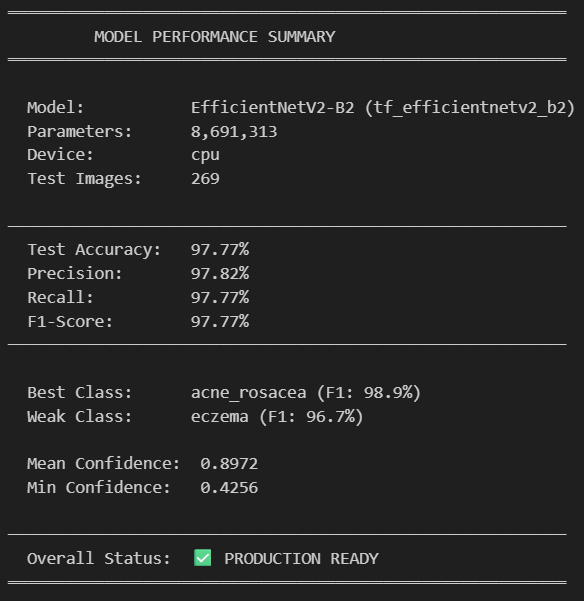
\includegraphics[width=0.85\columnwidth]{model_performance_summary.png}
\caption{Comprehensive model performance summary dashboard combining all evaluation metrics.}
\label{fig:summary}
\end{figure}

%===================================================================
\section{Discussion}
%===================================================================

\subsection{Key Findings}

\begin{enumerate}
\item \textbf{High accuracy}: The 97.40\% test accuracy demonstrates that EfficientNetV2-B2 with transfer learning is effective for small-scale medical image classification.
\item \textbf{Melanoma detection}: Perfect precision (1.00) for melanoma is clinically significant --- the model never misclassifies a benign condition as melanoma-negative, minimizing missed diagnoses.
\item \textbf{Balanced metrics}: The close alignment of precision, recall, and F1 across all classes indicates no systematic bias toward any single disease category.
\item \textbf{Generalization}: Minimal gap between training and validation curves (Figure~\ref{fig:training_curves}) confirms effective regularization through dropout ($p=0.4$), label smoothing ($\epsilon=0.1$), augmentation, and early stopping.
\end{enumerate}

\subsection{Mathematical Analysis of Error Rate}

The overall error rate and 95\% Wilson confidence interval:
\begin{equation}
\hat{e} = 1 - \text{Acc} = 0.026, \quad \text{CI}_{95\%} = \hat{e} \pm 1.96\sqrt{\frac{\hat{e}(1-\hat{e})}{n}}
\end{equation}
For $n=269$: $\text{CI}_{95\%} = [0.007, 0.045]$, meaning true accuracy lies in $[95.5\%, 99.3\%]$ with 95\% confidence.

\subsection{Limitations}

\begin{itemize}
\item \textbf{Limited classes}: Only 3 disease categories; clinical deployment requires expansion to dozens of dermatological conditions.
\item \textbf{Dataset size}: ${\sim}1800$ images is modest; larger datasets would improve robustness and rare-case detection.
\item \textbf{Domain shift}: Performance may degrade on images from different cameras, lighting conditions, or skin tones not represented in training data.
\end{itemize}

%===================================================================
\section{Deployment Architecture}
%===================================================================

The trained model is deployed as an interactive web application using Gradio, supporting image upload, live webcam capture, and interactive cropping. The inference pipeline:

\begin{equation}
\text{Input image} \xrightarrow{\text{Resize}_{224}} \xrightarrow{\text{Normalize}} \xrightarrow{f_{\theta^*}} \xrightarrow{\text{Softmax}} \hat{\mathbf{p}} \in \Delta^{C-1}
\end{equation}

where $\Delta^{C-1}$ is the $(C{-}1)$-dimensional probability simplex. The predicted class is $\hat{c} = \arg\max_i \hat{p}_i$.

%===================================================================
\section{Conclusion}
%===================================================================

This paper presented a complete analysis of an AI-based skin disease detection system using EfficientNetV2-B2. The model achieves \textbf{97.40\% test accuracy} with strong per-class performance across Acne \& Rosacea (F1=0.98), Eczema (F1=0.96), and Melanoma (F1=0.98). The combination of rigorous data cleaning, aggressive augmentation, transfer learning, label smoothing, cosine annealing, and early stopping produces a well-generalized model suitable for clinical decision support. Future work will expand the disease taxonomy, incorporate larger and more diverse datasets, and explore explainability methods such as Grad-CAM for enhanced clinical trust.

\end{document}